\documentclass[11pt, a4paper]{article}
\usepackage{sectsty}
\usepackage{enumitem}
\usepackage{graphicx}
\usepackage{amsmath}
\usepackage{amssymb}
\usepackage{setspace}
\usepackage{tasks}
\usepackage{graphicx}
\usepackage{float}
\usepackage{comment}
\usepackage{listings}
\usepackage[utf8]{inputenc}
\usepackage{amsfonts}
\usepackage{gensymb}
\usepackage{multicol}
\usepackage{tabularx}
\usepackage{tikz}
\newcommand{\myvec}[1]{\ensuremath{\begin{pmatrix}#1\end{pmatrix}}}
\let\vec\mathbf

\newcommand{\mydet}[1]{\ensuremath{\begin{vmatrix}#1\end{vmatrix}}}
\providecommand{\brak}[1]{\ensuremath{\left(#1\right)}}
\providecommand{\lbrak}[1]{\ensuremath{\left(#1\right.}}
\providecommand{\rbrak}[1]{\ensuremath{\left.#1\right)}}
\providecommand{\cbrak}[1]{\ensuremath{\left\{#1\right\}}}
\providecommand{\sbrak}[1]{\ensuremath{{}\left[#1\right]}}
\providecommand{\norm}[1]{\left\lVert#1\right\rVert}
\providecommand{\abs}[1]{\left\vert#1\right\vert}

\title{ \textbf{Math Computing}}
\author{ Chakali Suresh }
\date{}

\begin{document}
\vspace{-\baselineskip}
\maketitle

\section*{NCERT 9.7.1.7}

\textbf{This question is from class 9 ncert chapter 7.triangles}
\begin{enumerate}
	\item $AB$ is a line segment and $P$ is its mid-point. $D$ and $E$ are points on the same side of $AB$ such that $\angle BAD = \angle ABE$ and $\angle EPA = \angle DPB$. Show that
		\begin{enumerate}
	\item $\triangle DAP \cong  \triangle EBP$
	\item $AD = BE$
\end{enumerate}
\begin{figure}[H]
    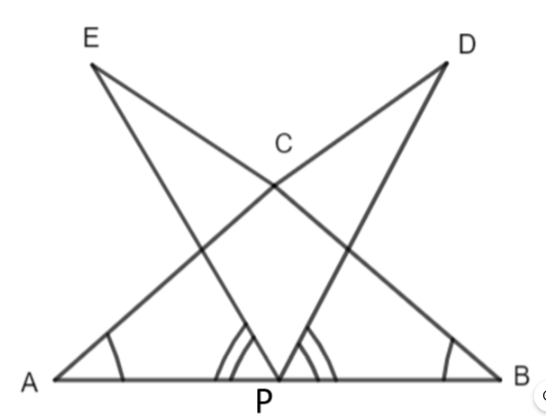
\includegraphics[width=\columnwidth]{figs/mc.png}
    \caption{$\triangle  DAP \hspace{12pt} and \hspace{12pt} \triangle EBP$}
 \label{fig:fig1}
\end{figure}
\pagebreak
\textbf{Construction steps:}
\\
		\begin{enumerate}[label=(\roman*)]
\item Let point $A$ be the reference point whose coordinates are at origin. 
\begin{align}
\vec{A} &= \myvec{0 \\ 0}
\end{align}

\item Let the distance between point $A$ and $B$ be $x$, and also considering the point $B$ on same axis .
\begin{align}
	\norm{A-B} &= x
\end{align}
 So,the coordinates of point $B$ be,
\begin{align}
\vec{B} &= \myvec{x \\ 0}
\end{align}

\item Given the point $P$ is the mid-point of line segment $AB$,
\begin{align}
	\vec{P} &= \myvec{\frac{A+B}{2}}\\
	\vec{P} &= \myvec{a \\ b}
\end{align}

\item Let the coordinate points of $D$ and $E$ are,
\begin{align}
\vec{D} &= \myvec{ x_1 \\ x_2},\\
\vec{E} &= \myvec{ x_3 \\ x_4}
\end{align}

\item Let assume the distance between point $A, D$ and $B, E$ be $r$ ,and the line $AB$ makes an angle $ \theta $ anticlock-wise from point $A$ clock-wise from point $B$ with the line $AD$ $BE$.
\begin{align}
	\norm{A-D} &= \vec{r} = \norm{B-E} \\
	\angle BAD &= \theta = \angle ABE
\end{align}

$\therefore$ Now the coordinates of point $D, E$ are,
\begin{align}
	\vec{D} &= \myvec{ x_1 \\ x_2 } = \myvec{r \cos \theta \\ r\sin \theta} \\
	\vec{E} &= \myvec{ x_3 \\ x_4 } = \myvec{-r \cos \theta \\ r \sin \theta} 
\end{align}

\item Similarly, the mid-point $P$ also makes an angle $\theta$ with the points $D$ and $E$
	\begin{align}
		\angle BAD &= \theta = \angle ABE
	\end{align}

\item Now the coordinates of $A,B,P,D$ and $E$ are ,
\begin{align}
\vec{A} &= \myvec{0 \\ 0},\\
\vec{B} &= \myvec{x \\ 0} ,\\
\vec{P} &= \myvec{a \\ b} ,\\
\vec{D} &= \myvec{r \cos \theta \\ r \sin \theta} \\
\vec{E} &= \myvec{-r \cos \theta \\ r \sin \theta} 
\end{align}

\item Let assume, 
\begin{align}
	x &= 5 \\
	r &=4 \\
	\theta_1 &= 30\degree(\text{for the angle BAD and ABE})\\
	\theta_2 &= 60\degree(\text{for the angle EPA and DPB})
\end{align}

\item on substituting the values,
\begin{align}
\vec{A} &= \myvec{0 \\ 0},\\
\vec{B} &= \myvec{5 \\ 0} ,\\
\vec{P} &= \myvec{2.5 \\ 0} ,\\
\vec{D} &= \myvec{4 \cos 30 \degree \\ 4 \sin 30 \degree },\\
\vec{E} &= \myvec{-4 \cos 30 \degree \\ 4 \sin 30 \degree },\\
\vec{D} &= \myvec{4 \cos 60 \degree \\ 4 \sin 60 \degree } ,\\
\vec{D} &= \myvec{-4 \cos 60 \degree \\ 4 \sin 60 \degree } 
\end{align}

\item on calculating we get  ,
\begin{align}
\vec{A} &= \myvec{0 \\ 0},\\
\vec{B} &= \myvec{5 \\ 0} ,\\
\vec{P} &= \myvec{2.5 \\ 0} ,\\
\vec{D} &= \myvec{ 3.464101 \\ 2 } ,\\
\vec{E} &= \myvec{-3.464101  \\ 2 },\\
\vec{D} &= \myvec{ -2 \\ 3.464101 } ,\\
\vec{E} &= \myvec{ -2 \\ 3.464101 }
\end{align}
Joining these points forms the required figure

\end{enumerate}
\end{enumerate}

\begin{figure}[H]
    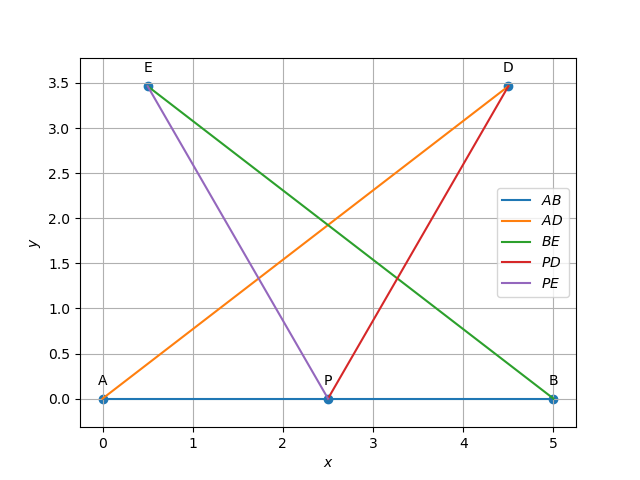
\includegraphics[width=\columnwidth]{figs/fig_mat_comp.png}
    \caption{$\triangle DAP \hspace{12pt} and \hspace{12pt} \triangle EBP$}
    \label{fig:fig2}
\end{figure}

\end{document} 
